% !TeX spellcheck = fr_FR

% TODO: Replace scan images with clean text where possible

\documentclass[a4paper, 10pt]{report}

\usepackage[french]{babel}
\usepackage[T1]{fontenc}

\usepackage{amsmath, amssymb, amsfonts}

\usepackage{hyperref}
\usepackage{geometry}

\usepackage{xcolor}
\usepackage{graphicx}

\usepackage{fancyhdr}
\usepackage{lastpage}

\usepackage{enumitem}

\geometry{
	a4paper,
	left=25mm,
	right=25mm,
	top=35mm,
	bottom=25mm,
	headsep=5mm,
	headheight=20mm,
}

\definecolor{solution}{HTML}{E5E4E2}
\providecommand{\abs}[1]{\lvert#1\rvert}
\providecommand{\norm}[1]{\lVert#1\rVert}
\DeclareMathOperator{\card}{card}

\begin{document}
	
	\renewcommand{\headrule}{%
		\vspace{-4pt}\hrulefill
		\raisebox{-6.8pt}{\ 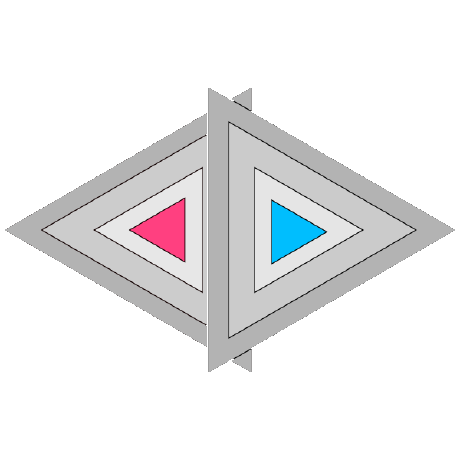
\includegraphics[height=5mm]{../../icon.png}}
		\hrulefill
	}	
	\pagestyle{fancy}
	\fancyhf{}
	
	\fancyhead[L]{\small \slshape Automne 2024}
	\fancyhead[C]{\Large \bfseries Algèbre I - Série 03}
	\fancyhead[R]{\small Buff Mathias}
	\fancyfoot[L]{
		\small Source files available at:
		\href{https://github.com/MathiasBuff/bsc-math}
		{github.com/MathiasBuff/bsc-math}
	}
	\fancyfoot[R]{
		\small Page \thepage
		\hspace{1pt} /
		\pageref*{LastPage}
	}
	

	\noindent
	\textbf{Exercice 1.} (Familles libres et génératrices de vecteurs)\\
	Les familles suivantes sont-elles libres ou génératrices ? Si oui
	le prouver, sinon donner un contre-exemple.
	
	\begin{enumerate}[label=\arabic*.]
		\item $\{(1, 1), (1, -i)\}$ dans l'espace vectoriel
		$\mathbb{C}^2$ sur $\mathbb{C}$
		
		\hspace*{-28mm}
		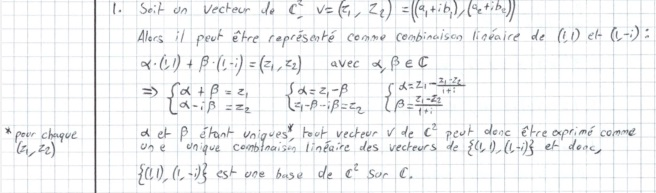
\includegraphics{ex01-p1.jpg}
		%
		\item $\{(1, 2, 2), (-2, 0, 2), (-2, 2, -1)\}$ dans l'espace
		vectoriel $\mathbb{R}^3$ sur $\mathbb{R}$
		
		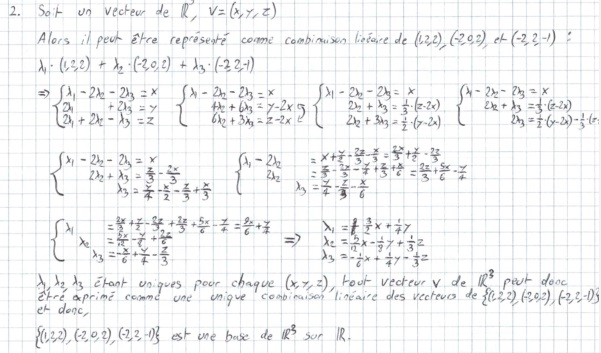
\includegraphics{ex01-p2.jpg}
		%
		\item $\{(1, 2, 2), (-2, 0, 2), (-2, 2, -1)\}$ dans l'espace
		vectoriel $\mathbb{C}^3$ sur $\mathbb{R}$
		
		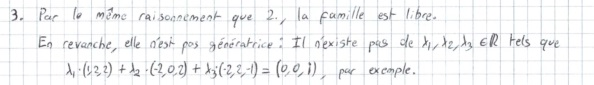
\includegraphics{ex01-p3.jpg}
		%
		\newpage
		\item Donner une base de $\mathbb{C}^2$ sur $\mathbb{R}$.
		Et sur $\mathbb{C}$ ?
		
		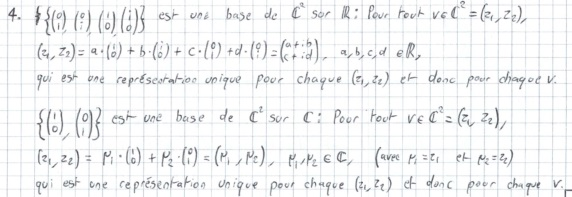
\includegraphics{ex01-p4.jpg}
	\end{enumerate}
	
	\fancyhf{}
	\renewcommand{\headrule}
	{\rule{\textwidth}{0pt}}
	\fancyfoot[R]{
		\small Page \thepage
		\hspace{1pt} /
		\pageref*{LastPage}
	}
	
	\vspace{5mm}
	\noindent
	\textbf{Exercice 2.} (Indépendance linéaire de fonctions)\\
	Dans l'espace vectoriel des fonctions
	$\mathcal{F}(\mathbb{R}, \mathbb{R})$, les familles ci-dessous
	sont-elles libres ?
	
	\begin{enumerate}[label=\arabic*.]
		\item $\{3x^2, 2x^4\}$
		%
		\item $\{3^x, 3^{x+3}\}$
		%
		\item $\{1, \sin^2(x), \cos^2(x)\}$
		%
		\item $\{\cos(x), \cos(2x), \cos(4x)\}$
		%
		\item La famille infinie $\{1, \sin(x), \sin(2x), \sin(4x),
			\sin(8x), \sin(16x), \dotsc\}$
	\end{enumerate}
	
	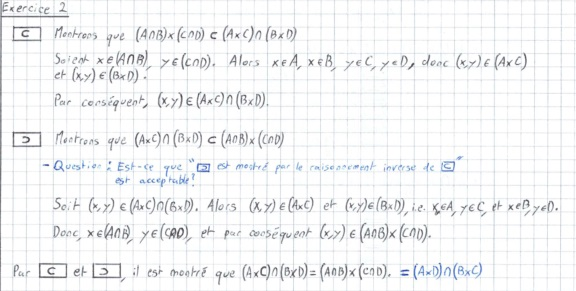
\includegraphics{ex02.jpg}
	
	\newpage
	
	\noindent
	\textbf{Exercice 3.} (Sous-famille libre)\\
	Montrer l'affirmation suivante :
	
	Si $\{v_1, \dotsc, v_n\}$ est une famille libre dans un espace
	vectoriel $V$,
	
	Alors toute sous-famille $\{v_i\}_{i \in I}$ indexée par 
	$I \subset \{1, \dotsc, n\}$ est aussi libre.\\
	
	\colorbox{solution}
	{
		\begin{minipage}{0.9\textwidth}
			Si $\{v_1, \dotsc, v_n\}$ est libre, alors pour tout
			$v_k, k \in K = \{1, \dotsc, n\}$, il est impossible de
			représenter $v_k$ comme combinaison linéaire des vecteurs
			de $\{v_1, \dotsc, v_n\} \setminus \{v_k\}$.\\
			
			En particulier, il est impossible de représenter $v_k$
			comme combinaison linéaire des vecteurs de n'importe quelle
			sous-famille de $\{v_1, \dotsc, v_n\} \setminus \{v_k\}$.\\
			
			Ainsi, pour tout $v_k$, une sous-famille $\{v_i\}_{i \in I},
			I \subset K$ contenant $v_k$ est libre. Comme $v_k$ peut
			être n'importe quel vecteur de $\{v_1, \dotsc, v_n\}$, on
			en conclut que toute sous-famille de $\{v_1, \dotsc, v_n\}$:
			$\{v_i\}_{i \in I}, I \subset \{1, \dotsc, n\}$ est libre.
		\end{minipage}
	}
	
	\vspace{5mm}
	\noindent
	\textbf{Exercice 4.} (Dimension d'un espace vectoriel sur
	$\mathbb{R}$ et sur $\mathbb{C}$)\\
	On note $\dim_{\mathbb{K}}(E)$ la dimension de l'espace vectoriel
	$E$ sur le corps $\mathbb{K}$.
	
	\begin{enumerate}[label=(\alph*)]
		\item Montrer que $\dim_{\mathbb{R}}(\mathbb{R}) = 1$ et
		$\dim_{\mathbb{R}}(\mathbb{C}) = 2$.
		%
		\item En déduire $\dim_{\mathbb{R}}(\mathbb{R}^n)$ et
		$\dim_{\mathbb{R}}(\mathbb{C}^n)$.
		%
		\item Montrer que $\dim_{\mathbb{C}}(\mathbb{C}) = 1$.
		En déduire $\dim_{\mathbb{C}}(\mathbb{C}^n)$.
	\end{enumerate}
		
	\colorbox{solution}
	{
		\begin{minipage}{0.9\textwidth}
			\begin{enumerate}[label=(\alph*)]
				\item - $\{1\}$ est une base de $\mathbb{R}$ sur
				$\mathbb{R}$, car $\forall v \in \mathbb{R},
					\exists! \lambda \in \mathbb{R},
					v = \lambda \cdot 1$.\\
				\phantom{- }Comme $\{1\}$ possède 1 élément,
				$\dim_{\mathbb{R}}(\mathbb{R}) = \card(\{1\}) = 1$
				
				- $\{1, i\}$ est une base de $\mathbb{C}$ sur
				$\mathbb{R}$, car $\forall v \in \mathbb{C},
				\exists! a \in \mathbb{R}, \exists! b \in \mathbb{R},
				v = a \cdot 1 + b \cdot i$.\\
				\phantom{- }Comme $\{1, i\}$ possède 2 éléments,
				$\dim_{\mathbb{R}}(\mathbb{C}) = \card(\{1, i\}) = 2$
				%
				\vspace{10pt}
				%
				\item - Puisqu'un vecteur de $\mathbb{R}^n$ est un
				n-uplet de vecteurs de $\mathbb{R}$, il peut être
				représenté comme\\
				\phantom{- }n vecteurs de $\mathbb{R}$ indépendants,
				et donc $\dim_{\mathbb{R}}(\mathbb{R}^n)
				= n \cdot \dim_{\mathbb{R}}(\mathbb{R}) = n \cdot 1 = n$.
				
				- Par le même raisonnement, $\dim_{\mathbb{R}}(\mathbb{C}^n)
				= n \cdot \dim_{\mathbb{R}}(\mathbb{C}) = n \cdot 2 = 2n$.
				%
				\item  $\{1\}$ est une base de $\mathbb{C}$ sur
				$\mathbb{C}$, car $\forall v \in \mathbb{C},
				\exists! z \in \mathbb{C}, v = z \cdot 1$.\\
				Donc, $\dim_{\mathbb{C}}(\mathbb{C}) = 1$ et
				$\dim_{\mathbb{C}}(\mathbb{C}^n)
					= n \cdot \dim_{\mathbb{C}}(\mathbb{C}^n)
					= n \cdot 1 = n$.
			\end{enumerate}
		\end{minipage}
	}
	
	\newpage
	
	\noindent
	\textbf{Exercice 5.} (Base, famille libre maximale et famille
	génératrice minimale)\\
	Soit $V$ un espace vectoriel sur $\mathbb{K}$ et une famille
	de vecteurs $\mathcal{F} = \{v_1, \dotsc, v_n\} \subset V$.
	
	\begin{enumerate}[label=(\alph*)]
		\item En cours, nous avons vu que les conditions suivantes
		sont équivalentes :
		\begin{enumerate}[label=(\roman*)]
			\item $\mathcal{F}$ est une base de $V$
			\item $\mathcal{F}$ est une famille
				libre maximale de $V$
			\item $\mathcal{F}$ est une famille
				génératrice minimale de $V$
		\end{enumerate}
		L'équivalence $(i) \iff (ii)$ a été montrée en cours.
		Montrer l'équivalence $(i) \iff (iii)$.
		%
		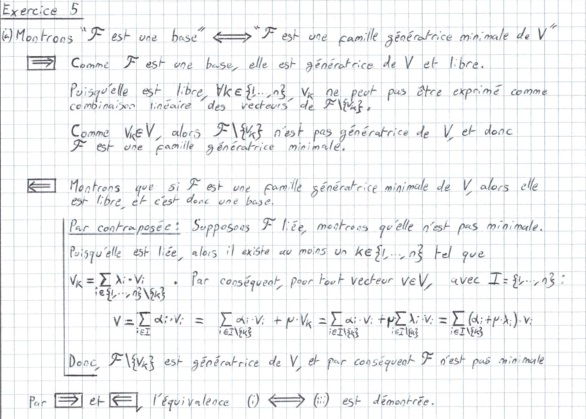
\includegraphics{ex05-p1.jpg}
		%
		\item Montrer que
		\[
			\mathcal{F}\ \text{est une base de}\ V \iff
			\mathcal{F}\ \text{est génératrice et}\
			\card(\mathcal{F}) = \dim_{\mathbb{K}}(V)
		\]
		\textit{Indication :} $card(\mathcal{F})$ est le nombre
		d'éléments de la famille $\mathcal{F}$.
		
		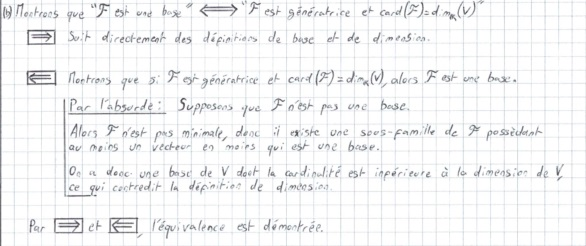
\includegraphics{ex05-p2.jpg}
	\end{enumerate}
	
\end{document}
